\vspace{1cm}

\itshape
En este capítulo se presenta el estado del arte del presente trabajo. Se pretende que el lector
conozca los avances que se llevaron a cabo en el estudio de topologías tolerantes a fallas,
tales como árboles binarios (Sección \ref{sec:binary_tree} página \pageref{sec:binary_tree}),
redes hypercube (Sección \ref{sec:hypercube} página \pageref{sec:hypercube}), redes distribuidas
(Sección \ref{sec:redes_distribuidas} página \pageref{sec:redes_distribuidas}), redes Ethernet
(Sección \ref{sec:ethernet} página \pageref{sec:ethernet}), arquitecturas basadas en bus
(Sección \ref{sec:bus} página \pageref{sec:bus}).

En la Sección \ref{sec:metrica_modelado} (página \pageref{sec:metrica_modelado})
las métrica y modelado de la confiabilidad de sistemas.

Para finalizar, en la Sección \ref{sec:CAN_space} (página \pageref{sec:CAN_space}) se comenta sobre
CAN en la actividad espacial.
\upshape

\noindent\rule{\textwidth}{2pt}

\vspace{1cm}

% section that explain binary tree
%TODO: Arboles binarios
\begin{comment}
 Bibliografía utilizada aquí:
 
 \cite{Raghavendra84} -> Fault tolerance in Binary Tree Architecture
 
\end{comment}


\section{Árboles binarios}\label{sec:binary_tree}
El concepto de arquitecturas de árboles binarios es aplicable en el desarrollo de sistemas de 
computadoras jerárquicas, y sobre todo en computadoras de alta perfomance \citep{Raghavendra84}. 
Existen dos diferentes mecanismos de tolerancia a fallas \citep{Raghavendra84}:
\begin{enumerate}
 \item Esquemas con back up.
 \item Esquemas con degradación de perfomance.
\end{enumerate}

Teniendo en cuenta que estas arquitecturas son aplicadas principalmente en la construcción de 
circuitos VLSI\footnote{Del inglés, Very Large Scale Integration} \citep{Singh91}, se asume su 
aplicabilidad a arquitecturas de aviónica. 

La \ac{FT} y la perfomance de los sistemas dependen de las capacidades de las redes que se utilizan 
para la comunicación entre unidades de procesamiento \citep{Raghavendra84}. 

Un árbol binario está compuesto por nodos y enlaces (links). Existe un nodo central dónde se 
desprenden dos nodos hijos, estos se encuentran enlazados al nodo padre. Así recursivamente, se 
van generando dos nuevos hijos, por cada uno de los nodos. Los árboles binarios están divididos en 
niveles, que representa cada una de las generaciones de nodos.

Este tipo de topología tiene algunos problemas que la \ac{FT} debe hacer frente. En las 
arquitecturas basadas en árboles binario, existe una cierta probabilidad de que un nodo o un link 
falle \citep{Raghavendra84}. Las arquitecturas de árbol binario son en general físicamente 
estáticas. Por lo tanto, cualquier falla en uno de sus nodos (o links) demandaría una avería a 
nivel sistema, lo cual daría lugar a una pérdida de misión. Para ello se debe dotar a la 
arquitectura de un mecanismo de reconfiguración.

La tolerancia a fallas en arquitecturas binarias ya fueron estudiadas en profundidad en 
\cite{Hayes76}, \cite{Raghavendra84}, \cite{Singh91}. Para lograr \ac{FT} en estas arquitecturas se 
las deben diseñar con un número mínimo de nodos de backup y links redundantes, de modo tal de hacer 
frente cualquier punto de falla simple en la arquitectura. 

\subsection{Esquema de árbol binario con backups}
El esquema planteado por \cite{Raghavendra84} es similar al que se muestra en al Figura 
\ref{fig:binary_tree}. En este esquema se agregan nodos y links redundantes como técnica de \ac{FT}. 
Existe un nodo de backup por cada nivel del árbol.

\begin{figure}[h]
 \centering
 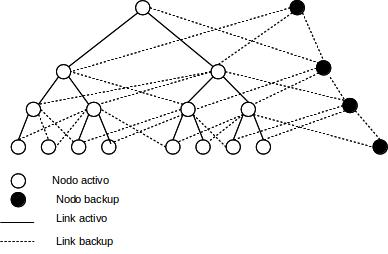
\includegraphics[scale=1]{images/Marco_teorico/binary_tree}
  \caption{Árbol binario de 4 niveles}  
\label{fig:binary_tree} 
\end{figure}

Esta arquitectura cuenta con una restricción, la cual indica que solo se puede tolerar una 
falla singular, por cada nivel de la arquitectura. Arquitecturas de este tipo, podrían tolerar más 
de una falla, sólo si se dan en diferentes niveles del árbol \citep{Raghavendra84}. Para agregar 
más tolerancia, se deberían agregar más redundancias.

Notese en la Figura \ref{fig:binary_tree} que cuando una unidad de procesamiento (nodo) falla, 
todos los links se deben reajustar hacia el nodo de la derecha. En este punto es importante 
mencionar, que ante esta situación se requiere una reconfguración a nivel de \ac{HW}, además de una 
reconfiguración a nivel de \ac{SW}. Es necesario algoritmos de ruteo dinámicos, de modo tal de 
conocer los nuevos caminos que intercomunican nodos, para mantener la operabilidad del sistema.  

\subsubsection{Estimación de la confiabilidad de un árbol binario con backup}\label{subsec:conf_binary_tree}
Se asume que la probabilidad de fallas de los links es muy baja en comparación con la de los nodos. 
Teniendo que el rate de falla es de $\lambda$, la confiabilidad  de un nodo es $R = e^{-\lambda 
t}$. También se sabe que un árbol binario con n niveles,  tiene $2^n - 1$ nodos en total. 
Entonces la confiabilidad de todo el sistema es: $$R_{nr} = R^{2^n - 1}$$

\cite{Raghavendra84} incluye en sus cálculos un factor de cobertura $c$, el cual es la probabilidad 
condicional de que se lleve a cabo una recuperación exitosa, luego de que una falla se haya 
detectado. Entonces la confiabilidad del sistema para una arquitectura de árbol binario con 
redundancias (un nodo backup por nivel) es el siguiente: $$R_{sys} = \prod_{k=0}^{n-1}{[R^{2k +1} + 
R^{2k}(1-R) + 2^kcR^{2k}(1-R)]}$$.

Simplificando: $$R_{sys} = R^{2n +1} \prod_{k=0}^{n-1}{[(2^kc+1) - 2^kcR]}$$

En la Figura \ref{fig:Reliability_binary_tree_4_levels}, se observa la confiabilidad de una 
arquitectura de árbol binario de 4 niveles, con una cantidad de $2^4 -1 = 15$ nodos. En color negro 
se grafica una arquitectura sin redundancia, mientras que en color rojo, azul y cyan, se muestra 
arquitecturas redundadas con diferentes $c$ (0.98, 0.99, 1, respectivamente). 

\begin{figure}[h]
 \centering
 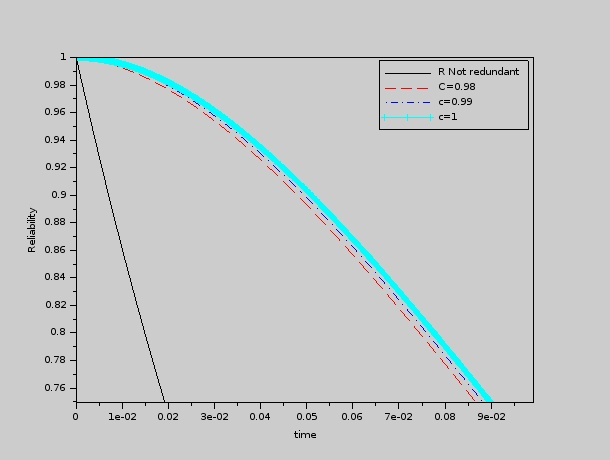
\includegraphics[scale=0.5]{images/Marco_teorico/Reliability_binary_tree_4_levels.jpg}
  \caption{Confiabilidad con respecto al tiempo de una arquitectura de árbol binario de 4 niveles}  
\label{fig:Reliability_binary_tree_4_levels} 
\end{figure}

Con esto podemos indicar, como es de esperarase, una arquitectura de árbol binario redundanda 
permite mantener un alto nivel deseable de confiabilidad, durante un mayor lapso de tiempo, a 
diferencia de un sistema no redundando. También se puede concluir que con un factor de cobertura $c$
más próximo a uno, maximiza los niveles de confiabilidad con respecto al tiempo. 

%\subsubsection{Extensión de la arquitectura con backup}

%\subsection{Esquema de árbol binario con degradación de perfomance}

% section that explain the hypercube systems
\section{Sistemas Hypercube}
Hypercube es una técnica utilizada para
conectar múltiples procesadores. Esta topología
tiene propiedades de tolerancia a fallas de un
componente, ya que si esto se produce, no se
transmite a todo el sistema \citep{Rong96}. Otra ventaja que
presenta esta topología es la disponibilidad de
enlaces entre cualquier par de nodos \citep{Mostafa14}. Un
hypercube n-dimensional tiene: $$2^n $$ nodos y $$n2^{n-1}$$ enlaces.
Los nodos está conectados a n nodos vecinos a través de n enlaces \citep{Rong96}. Estas
relaciones pueden ser representadas en forma de matrices de proximidad \citep{Mostafa14}.
En \cite{Mostafa14} se muestra una manera sencilla de calcular la confiabilidad
de sistemas de este tipo. La probabilidad de falla de la red ($p_n$) depende
de la probabilidad de falla de cada uno de los nodos ($p_n$), suponiendo
que todos los nodos tienen la misma probabilidad de falla la confiabilidad
del sistema sería: $$R(N) = 1 -(NP_v)$$.

Para calcular la confiabilidad de una red hypercube se debe seguir
la fórmula $$R(N) = 1 -(NP_v)$$, a esta se le realiza leves modificaciones
para obtener el siguiente cálculo de confiabilidad: $$ R_{sys} = 1 - [N(1-e^{- \lambda t})]$$

% section that explain Distributed network
\section{Redes distribuídas}
Una red de computadoras hace referencia a un conjunto de computadoras autónomas que se encuentran interconectadas, esto quiere decir que pueden intercambiar información \citep{Tanenbaum12}. Una red distribuída tiene como principal caraceterística que no existe un nodo central que "gestione" toda la red. Todas las cargas de las tareas y/o actividades son distribuídas entre los nodos que forman parte de la red.

Una red distribuída es tolerante a fallas si los nodos pueden formar subredes \citep{Stivaros92}. Es decir, la red se debe mantener activa y conectada, con diferentes topologías e interconexiones, que permitan tolerar posibles fallas producidas en algunos nodos y permitir mantener la perfomance \citep{Stivaros92}. Debido a que el procesamiento de la red se encuentra distribuída en todo el sistema, esto brinda una ventaja por encima a los sistemas centralizados desde el punto de vista de la confiabilidad \citep{Pradhan82}. Un componente importante de las redes distribuídas tolerantes a fallas, es la topología del sistema \citep{Pradhan82}.

Siguiendo la notación de \cite{Pradhan82} para describir la topología del sistema se utiliza, un gráfico sin direccionamiento G = <V,E>, donde V representa un set de nodos y E representa un set de relaciones. \cite{Stivaros92} agrega que $V(G) = \{v_1,v_2,v_3, ... v_n \}$ representa un vector de nodos, los cuales tiene probabilidades de operación $P = (p_1, p_2, p_3, p_n)$; y define una función de asignación $\pi$, la cual es una función que asigna V con una probabilidad $P_{\pi(v)}$.

La \ac{FT} de la red G, dado el vector de probabilidades \vec{P} y una función de asignación $\pi$, tal como se viene discutiendo anteriormente, es la probabilidad de que la red continúe funcionando, es decir continúe conectada, aún en la falla (aleatoria) de alguno de sus nodos, esto se denota $FT(G;\vec{P},\pi)$.

Se dice que un subset de nodos S, es un estado tolerante del sistema G, cuando estos nodos se mantienen conectados y funcionales. Se utiliza $\theta$ para indicar el conjunto de todos los S posibles. Un estado tolerante S contribuye $\prod_{v\in S}{P_{\pi (v)}} \prod_{v \notin S} (1-p_{\pi (v)})$ a la probabilidad de \ac{FT}.

Para calcular el total de la \ac{FT} del sistema, incluyendo todo los S, se hace: $$FT(G;\vec{P};\pi) = \sum_{S \in \theta}{Pr(S)} = \sum_{S \in \theta}{\prod_{v\in S}{P_{\pi (v)}} \prod_{v \notin S} (1-p_{\pi (v)})}$$

Una relación entre nodos es representado  como ij, lo cual representa un enlace bidireccional entre nodos. El grado del nodo i representa el número de relaciones que inciden en ese nodo, el cual se escribe $d_i$. Así, $d_i$ está limitado por el número de puertos de entrada y salida disponibles por cada nodo \citep{Pradhan82}. $k_{ij}$ representa el número mínimo de \textit{hop} (hop representa la transmisión a través de un link de datos)\citep{Pradhan82}

\cite{Stivaros92} y \cite{Pradhan82} mencionan la existencia de varias topologías que pueden ser aplicadas en una red distribuída tolerante a fallas. Una topología estrella posee una baja distancia entre nodos, pero una pobre tolerancia a fallas \citep{Pradhan82} \citep{Stivaros92}. La topología anillo, permite un simple ruteo, pero existen grandes distancias internodo. Un sistema completamente interconectado, presenta buenas características tolerantes a fallas, pero tiene un alto costo \citep{Pradhan82}. \cite{Pradhan82} propone una topología para una arquitectura distribuída de comunicación. Esta es una topología robusta, y puede llegar a ser compleja a medida que aumentan los nodos.

\subsection{Algoritmo de ruteo}
Los algoritmos de ruteos son necesarios en el desarollo de una arquitectura tolerante a fallas y reconfigurable. Los algoritmos de ruteo se los pueden dividr en dos: \textit{algoritmos primarios} y \textit{algoritmo alternativo}. El primero es utilizado cuando no hay fallas de nodos. Se deben mantener los caminos para llegar, correctamente, al nodo destino. El segundo se utiliza en la presencia de alguna falla, este requiere que sea capaz de detectar la presencia de fallas, para luego reconfigurar el sistema. Estos algoritmos deben ser simples y requerir una mínima cantidad de \ac{HW} y \ac{SW}.

Agregado a lo mencionado en el párrafo anterior, deben existir algoritmos de diagnóstico distribuído de falas, basados en los algoritmos de ruteo \citep{Pradhan82}.

% section that explain Ethernet Network
\section{Redes Ethernet en aviónica}\label{sec:ethernet}
TTEthernet es una tecnología de red de computadoras comercializada por TTTech Computertechnik AG para el desarrollo de aplicaciones seguras. SAE International\footnote{http://www.sae.org} estandarizó esta red como SAE AS6802. TTEthernet se basa en el Ethernet clásico, en el cual se pone énfasis en las características principales que deben respetarse en sistemas críticos, tales como latencias de mensajes determinísticos, presición de tiempo real, tolerancia a fallas \citep{Loveless15}. Tiene la capacidad de transmitir datos 100 veces más rápido que la que lo hacen las tecnologías tradicionales tales como el MIL-STD-1553.

El Ethernet clásico presenta ventajas, tales como su alta velocidad de transmisión de datos, flexibilidad, y su disponibilidad y bajo costo (ya que se trata de un componente COTS) \citep{Loveless15}, hacen deseable su aplicación en el área espacial. Fue utilizado en diferentes proyectos aeroespaciales y en misiones importantes tales como el Space Shuttler y la Estación Espacial Internacional (ISS) \citep{Loveless15}. A pesar de esto, el Ethernet no cumple con el determinismo requerido por las aplicaciones de tiempo real de un vehículo espacial. Por tal motivo, se desarrolla el sistema TTEthernet, el cual introduce un reloj de sincronización descentralizado, permitiendo la transmisión de mensajes \ac{TT}. En este tipo de red, existe una herramienta de planning que asigna a cada dispositivo un intervalo de tiempo, en el cual puede utilizar para transmitir frames. Estos sistemas utilizan Links Virtuales (VL) para permitir el envío de mensajes time-trigged. Cada VL es asociado con un time-trigged frame através de un identificador de tráfico crítico (CTID), este reemplaza el control de acceso al medio (MAC) \citep{Loveless15}. Una red simple se muestra en la Figura \ref{fig:Arq_TTEthernet}.

\begin{figure}[h]
 \centering
 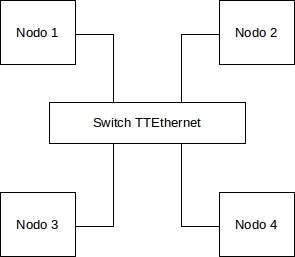
\includegraphics[scale=0.7]{images/Marco_teorico/TTEthernet_BUS.jpg}
  \caption{Arquitectura básica TTEthernet}
\label{fig:Arq_TTEthernet}
\end{figure}

TTEtheret puede actuar en dos clases de tráfico, con el objetivo de soportar diferentes niveles de cricticidad de mensajes. Estas clases de tráficos son las siguientes \citep{Loveless15} \citep{Steiner13}:
\begin{itemize}
	\item Time-Triggered, permite enviar mensajes de acuerdo a una planificación predefinida (scheduling),
	\item Rate-Constrained (RC), en el cual se llevan algunas restricciones de tamaño y rate de transmisión de frames,
	\item Best-Effort (BE), el cual se comporta de manera similar que el Ethernet
\end{itemize}

El paquete TTEthernet tiene una gran similitud con el frame del estándar IEEE 802.3 (Ethernet). Se denota en la Figura \ref{fig:Frame_TTEthernet} que en lugar de la MAC del 802.3 frame se divide en el CT Marker y el CTID. El primero es un identificador estático utilizado para distinguir paquetes \ac{TT} de otros tipos de tráficos.

\begin{figure}[h]
 \centering
 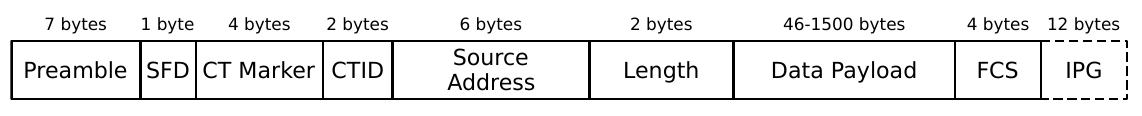
\includegraphics[scale=0.3]{images/Marco_teorico/Frame_TTEthernet.png}
  \caption{Frame de mensaje TTEthernet}
\label{fig:Frame_TTEthernet}
\end{figure}

El estándar SAE AS6802 define el protocolo de sincronización del TTEthernet. El protocolo TTP fue diseñado para reducir la complejidad de las arquitecturas distribuidas tolerantes a fallas \citep{TTTechWeb}. Existe un grupo de dispositivos de relojes locales que permite la sincronización requerida por la comunicación \ac{TT}, a esto se lo denomina \textif{dominio de sincronización} \citep{Loveless15}. Cada dominio de sincronización es asignado a uno de los siguientes roles:
\begin{itemize}
	\item Compression Master (CM)
	\item Synchronization Master (SM)
	\item Synchronization Cliente (SC)
\end{itemize}

\subsection{Experiencia de vuelo}
\cite{Loveless15} demuestra la aplicación de esta tecnología para computadoras de vuelo redundantes en misiones de naves simuladas. Esta tecnología toma tanto interés que el Sistema de Exploración Avanzada (AES)\footnote{Del ingles, Advanced Exploration Systems} de la \ac{NASA} lleva a cabo un proyecto denominado Avionics and Software (A&S). TTEthernet también fue utilizada en una arquitectura tolerante a fallas en el Integrated Power, Avionics and Software (IPAS)  del Johnson Space Center (JSC) y en el Core Flight Software (CFS) del Asteroid Redirect Mission (ARM) simulado\footnote{Los mencionados anteriormente son ejemplos de la utilización de TTEthernet} \citep{Loveless15}. También fue utilizado exitosamente durante la misión Orion \citep{TTTechOrion} .
TTEthernet simplifica el diseño de sistemas espaciales que deben contar con tolerancia a falla y una alta disponibilidad. La seguridad y la redundancia se mantiene sin ningún tipo de aplicación extra.

% section that explain the Bus network architecture
 \section{Arquitectura de red basada en BUS}
En \cite{Tai99} se presenta una arquitectura tolerante a fallas basada en BUS. Esta topología forma parte de un programa denominado X2000, el cual tiene como objetivo desarrollar una arquitectura tolerante a fallas y basada en componentes COTS. la cual pertenece a \ac{NASA}. Esta este programa se desarrolla bajo una filosofía de misiones espaciales la cual dice: "Más rápido, mejor, más económica" \footnote{En ingles, faster, better, cheaper}.

Esta arquitectura utiliza una topología novedosa denominada \textit{stack-tree topology} \citep{Chau99} \citep{Tai99}. Una stack-tree es un árbol donde cada nodo rama se encuentra conectado como mucho a tres otros nodos de los cuales, como máximo, dos son nodos ramas \citep{Tai99}. Una \ac{CST} es aquella en donde cada nodo rama está conectado al menos 1 nodo rama \citep{Tai99}.

En las Figura se pueden observar ejemplos de stack-tree. Mientra que en esta otra Figura no es una stack-tree.
\todo[inline]{Colocar las imagenes del paper BUS network architecture}

Como el objetivo principal es desarrollar una arquitectura tolerante a fallas, esto es, que aún cuando un nodo o un link entre nodos falle, el sistema completo debe continuar funcionando, sin ningún tipo de degradación en su servicio. Para cumplir con este objetivo \cite{Tai99} trabajan con un esquema de denominado \ac{CST} de equema dual (\ac{CST}$_D$) \footnote{En ingles,\ac{CST} dual scheme}. Esta puede observarse en la Figura
\todo[inline] {Colocar la imagen del paper, sonbre CSTd}

Para aumentar la confiabilidad de la arquitectra ante la acurrencia de fallas, se agrega links de backups que unen los nodos iniciales con el final, dando un efecto 3D de anillo \citep{Tai99}.

\subsection{Evaluación de la confiabilidad de arquitecturas basadas en BUS}
La confiabilidad de esta arquitectura (como ya se viene mencionando) es la probabilidad de que, a lo largo del tiempo de vida de la misión $t$, la arquitectura se encuentra funcional, en la cual todos los nodos (aquello que no hayn fallado) se encuentren conectados \citep{Tai99}. \citep{Tai99} y \citep{Chau99} asumen que la probabilidad de que un nodo falle es mucho mayor a que un enlace (el bus físico) falle.

En \cite{Tai99} indica que la confiabilidad de la red depende del tamaño $k$ (k es el número de nodos ramas). La confiabilidad de una red basada en \ac{CST} simplex es la probabilidad $U(k)$ de que los nodos no fallen, o que ante una falla se detecte y se lleve a cabo correctamente la reconfiguración del sistema. $$U(k) = (1-q) \sum_{j=0}^{k} {k}\choose{j} (1-q)^{k-j} (cq)^j $$ donde $q = 1-e^{-\lambda t}$ es la probabilidad de que un nodo falle durante el tiempo de vida de la misión $f$. Entonces $$R_s^{CST} = \sum_{k=1}^n (n-k+1)U(k)(cq)^{2(n-k)}$$ donde $(cq)^{2(n-k)}$ es la probabilidad que los  $2(n-k)$ nodos que conforman un cluster fallan, y esta falla es detectada y se lleva a cabo una correcta reconfiguración.

Para un \ac{CST} dual ocurre de manera similar. Se define $V(k)$ de la siguiente manera: $$V(k) = s(1-q)^k \sum_{j=1}^k {k}\choose{j} (1-q)^{k-j} (cq)^q + (1-q)^{2k}$$

Entonces la medida de $R_D^{CST} =  \sum_{k=1}^n (n-k+1) V(k) (cq)^{2(n-k)}$

% section that explain the modeling and metrics for critical system
\section{Métrica y modelado de la confiabilidad de sistemas}
Es de suma importancia llevar a cabo el análisis de la confiabilidad, disponibilidad y mantenibilidad (RAM\footnote{Del ingles, Realibility, Availability, Maintainability) de sistemas satelitales, durante la fase de diseño \citep{Hoque15}. Llevar a cabo esto, es de gran importancia, ya que permite el desarrollo de estrategias que permitan altos grados de confiabilidad, disponibilidad y mantenibilidad \citep{Hoque15}.

Existen dos categorías de medición de la confiabilidad y predición \citep{Schneidewind97}, estas son utilizadas para asegurar la seguridad del software de sistemas críticos \citep{Schneidewind97}, las cuales son:
  \begin{itemize}
    \item medición y predicción que están asociadas con las fallas y errores residuales.
    \item medición y predicción que están asociadas con la disponibilidad del sistema a sobrevir durante la misión sin experimentar fallas en el fallas (o pérdidas) en el sistema.
  \end{itemize}

  Las dos categorías mencionadas anteriormente son explicadas en \cite{Schneidewind97}.

  Según \cite{Liu14} las severidades de las fallas son clasificadas como críticas, peligrosas o triviales, teniendo en cuenta la contribución de esa falla a la pérdida de la misión. Es importante, además, conocer el riesgo de una falla. El riesgo, se define como la posibilidad de que una falla produzca una lesión (por ejemplo, un astronauta en vuelos tripulados), algún daño material (por ejemplo, la destrucción del satélite), o una pérdida (por ejemplo, la pérdida de la misión).

  Dependiendo de la misión, un criterio para definir si un sistema es seguro o no, es reduciendo las fallas que pueden provocar pérdidas de vida, pérdida de la misión o la obligación de abortar una misión \citep{Schneidewind97}. \cite{Schneidewind97} define dos criterios que deben satisfacerse:
  \begin{itemize}
    \item $r(t_t) < r_c$,
    \item $T_F(t_t) > t_m$
  \end{itemize}

  dónde $t_t$ es el Tiempo total de testing (observado o predicto); $r(t_t)$ son las fallas restantes hasta $t_t$; $r_c$ es una valor crítico de fallas restantes ;$T_F(t_t)$ es la métrica para medir el riesgo; y $t_m$ es la misión de la duración.

  Lo anterior signifca que un sistema crítico será seguro si: las fallas restantes en el tiempo de prueba son menores a un valor crítico de cantidad de fallas, o la duración de una misión es mayor al tiempo que se de la siguiente falla.
  
 En la literatura se utilizan modelos matemáticos para modelar los sistemas críticos y calcular así su confiabilidad. La mayoría de ellos asumen, que todas las fallas tienen igual tasa de detección de fallas, como así también la misma severidad, lo cual no es correcto \cite{Liu14}.

% section that explain the uses of CAN in space activity
\section{CAN en la actividad espacial}
CAN ya es utilizado en misiones satelitales, pero en la mayoría de los
casos es utilizado como bus secundario de comunicación, dejando el bus
primario para otros medios de comunicación más clásicos como el
MIL-STD-1553B.

La Agencia Espacial Europea (ESA) es la principal organización que se
esfuerza en desarrollar hardware, firmware y software que implementa
CAN como sistema de comunicación y control a bordo de vehículos espaciales.
Esta organización definió el estándar ECSS-E-ST-15C con el objetivo de
estandarizar el protocolo de comunicación CAN. La ESA observa que existe
una tendencia de producir un cambio de  paradigma 
centralizado, a funciones autónomas distribuidas, además, tiene en cuenta las ventajas que
brinda CAN para el desarrollo de satélites. Por ello, lleva a cabo anualmente
el \textit{CAN in Space Workshop}\footnote{https://indico.esa.int/indico/event/162/}.

Debe destacarse que CAN tiene vasta experiencia de vuelo en aviónica de
vehículos aereos (helicopteros y aviones). Lo cual alienta su aplicación
en la industria espacial.


\vspace{1cm}
\noindent\rule{\textwidth}{2pt}

\textbf{\Large{Resúmen}}

Un \textbf{árbol binario} está compuesto por nodos y enlaces (links). Existe un nodo central dónde se 
desprenden dos nodos hijos, estos se encuentran enlazados al nodo padre. Así recursivamente, se 
van generando dos nuevos hijos, por cada uno de los nodos. Los árboles binarios están divididos en 
niveles, que representa cada una de las generaciones de nodos. Para lograr \ac{FT} en estas arquitecturas se las deben diseñar con un número mínimo de nodos de backup y links redundantes, de modo tal de hacer frente cualquier punto de falla simple en la arquitectura.

\textbf{Hypercube} es una técnica utilizada para
conectar múltiples procesadores. Esta topología
tiene propiedades de tolerancia a fallas de un
componente, ya que si esto se produce, no se
transmite a todo el sistema. Otra ventaja que
presenta esta topología es la disponibilidad de
enlaces entre cualquier par de nodos.

Una \textbf{red distribuida} tiene como principal caraceterística que no existe un nodo central que ``gestione'' toda la red. Todas las cargas de las tareas y/o actividades son distribuidas entre los nodos que forman parte de la red. Una red distribuída es tolerante a fallas si los nodos pueden formar subredes. Es decir, la red se debe mantener activa y conectada, con diferentes topologías e interconexiones, que permitan tolerar posibles fallas producidas en algunos nodos y permitir mantener la perfomance.

\textbf{TTEthernet} es una tecnología de red de computadoras comercializada por TTTech Computertechnik AG para el desarrollo de aplicaciones seguras. SAE International estandarizó esta red como SAE AS6802. TTEthernet se basa en el Ethernet clásico, en el cual se pone énfasis en las características principales que deben respetarse en sistemas críticos, tales como latencias de mensajes determinísticos, presición de tiempo real, tolerancia a fallas. Tiene la capacidad de transmitir datos 100 veces más rápido que la que lo hacen las tecnologías tradicionales tales como el MIL-STD-1553.

Para medir la confiabilidad y, que es utilizada para
asegurar la seguridad del software de sistemas críticos, existen dos categorías
\begin{itemize}
    \item[-] medición y predicción que están asociadas con las fallas y errores residuales.
    \item[-] medición y predicción que están asociadas con la disponibilidad del sistema a sobrevivir durante la misión sin experimentar fallas (o pérdidas) en el sistema.
\end{itemize}

Por útlimo en este capítulo se comenta que el protocolo de comunicación
\textbf{CAN} ya es utilizado en misiones satelitales, pero en la mayoría de los
casos es utilizado como bus secundario de comunicación, dejando el bus
primario para otros medios de comunicación más clásicos como el
MIL-STD-1553B.

La ESA observa que existe
una tendencia de producir un cambio de  paradigma 
centralizado, a funciones autónomas distribuidas, además, tiene en cuenta las ventajas que
brinda CAN para el desarrollo de satélites. Por ello, lleva a cabo anualmente
el \textit{CAN in Space Workshop}
